\section*{Test 15  Movement of a large crowd of pedestrians around a corner}

Test 15 aims to demonstrate the extent to which the movement of persons around a corner affects the calculated evacuation time. Construct three geometries as illustrated in Figure 16 below. Locate 500 persons in the with "start" marked areas. The same group of persons should be chosen for each geometry so that the initial conditions are identical for all three geometries. The destination area is marked with "target".


\noindent
By comparing the results (time taken for all persons to reach the destination) it can be determined how much a corner influences the simulation result, as the right illustration represents the shortest route and the illustration on the left is the longest. Ideally, the result from the “corner” will be in between the two results for the shortest and longest straight-line route.



\begin{figure}[h]
	\centering
	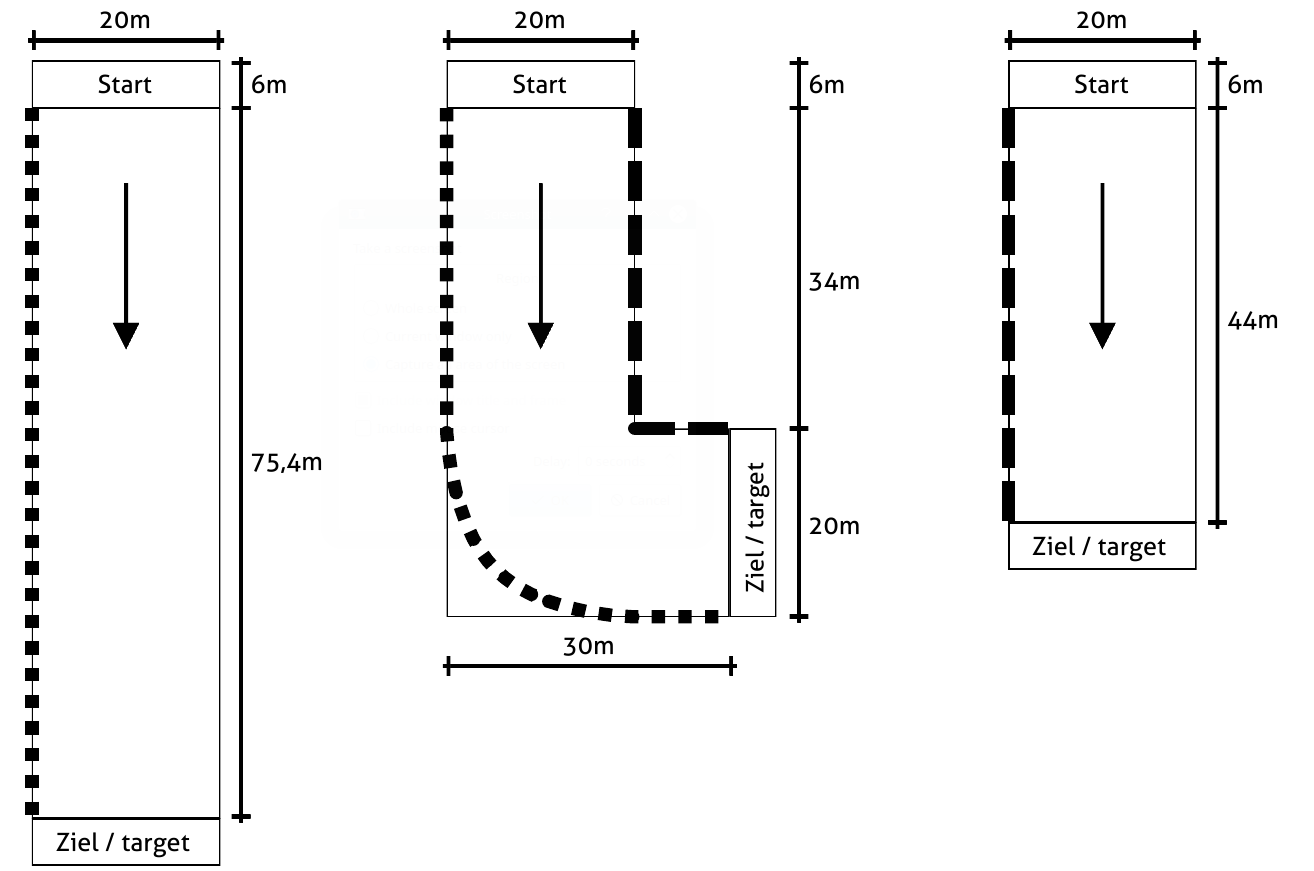
\includegraphics[scale=0.40]{test_description/Corridor_test_15.png}
	\caption{\footnotesize \textbf{Influence of a corner in the evacuation time. The lines with indentical style show the same lenght in different configurations.}}
\end{figure}
